\section{PACE methodology} 
\label{sec:method} 
Figure~\ref{fig: architecture} depicts the architecture: the supervised branch and the two sets of target-local branches feeding the final decision. Algorithm~\ref{alg: pace} describes the data processing performed prior to scoring and the steps at inference; further details on the scoring functions and choice of quantiles follow.



\begin{figure}[!htbp] 
\centering 
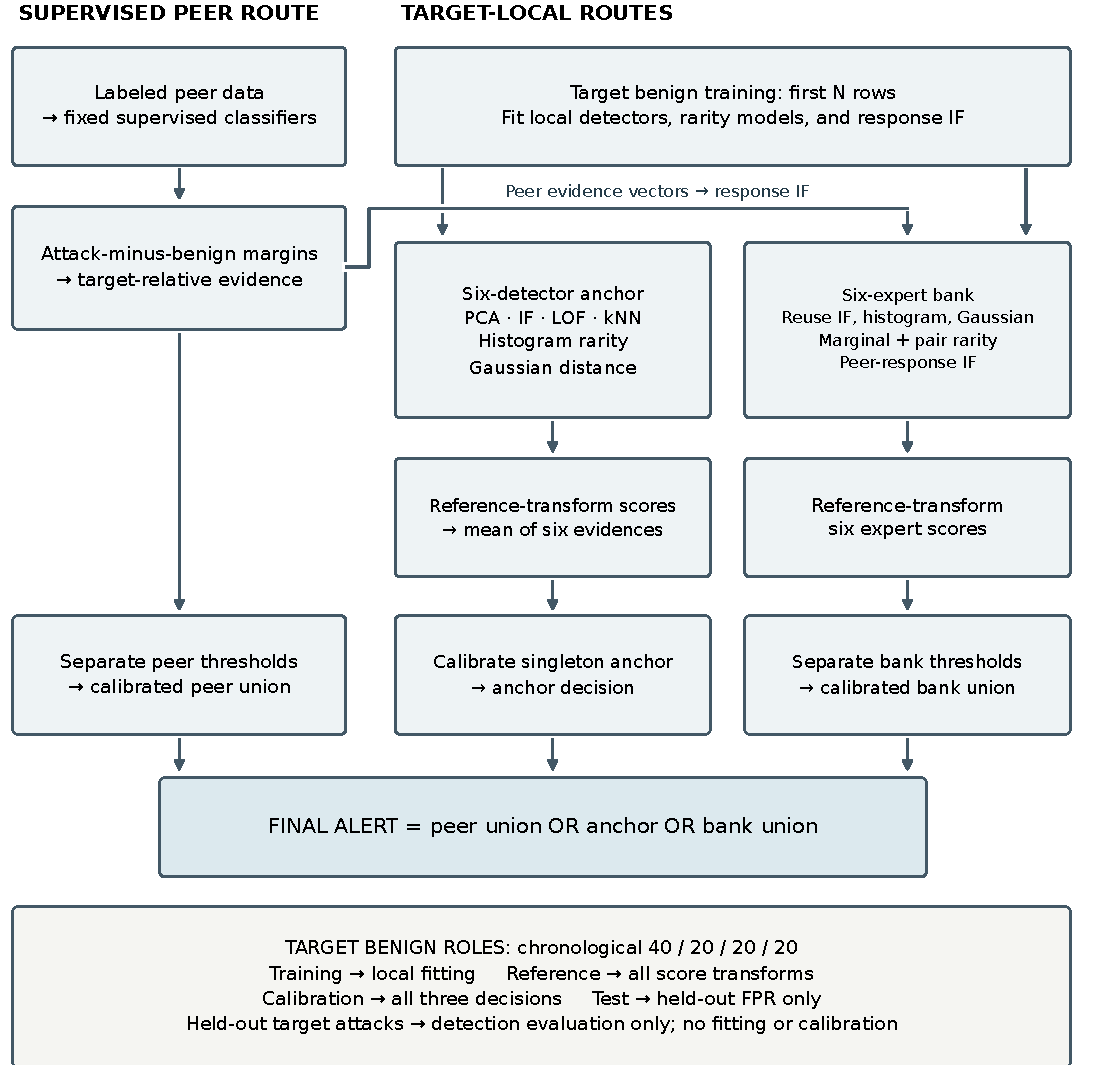
\includegraphics[width=0.88\textwidth]{figures/architecture.pdf} 
\caption{PACE architecture and final decision. Benign target training set, target reference, calibration, and test roles. Features are scaled using all fully-available target benign training roles, and local components fit on the restricted size $N$ target training roles. Attack labels are used only for scoring the detected attacks. IF = isolation forest, LOF = local outlier factor, kNN = $k$-nearest neighbours.}
\label{fig:architecture} 
\end{figure} 
\FloatBarrier 

\subsection{Target-relative evidence} 
Given an expert score $s$ with corresponding target reference scores $r_1,...,r_n$ and maximum $r_{\max}$, define $d_R=\max(r_{\max}-\textrm{median}_i r_i, 10^{-6})$, and
\begin{equation} 
E_R(s)=\begin{cases} 
-\log((1+\sum_{i=1}^n \mathbf{1}(r_i\ge s))/(n+1)), &s \le r_{\max}\\ 
\log(n+1)+\log(1+(s-r_{\max})/d_R) &s > r_{\max} 
\end{cases} 
\label{eq:evidence} 
\end{equation} 
which we adopt in our implementation. We include tied values in this computation. Scores exceeding the reference maximum are assigned to this score extrapolation instead of being treated as tied. Note that this latter step does not constitute a principled tail estimation procedure with any guarantees of accuracy. Each peer score yields an evidence score $e_k(x) = E_{R,k}(m_k(x))$.



\subsection{Blocks and quantiles} 
Given the number of calibration samples $M = |C|$ and our parameter $b=250$, the implementation constructs $\lfloor M/b\rfloor$ (at least 1) contiguous blocks via a NumPy balanced-split operation (i.e. block sizes will be no more than 1 apart, and preceding blocks take remaining samples if evenly divisible by $b$ is impossible -- these should thus not be interpreted as blocks of exactly 250, e.g. with 350 samples there would be 1 block of size 350). Letting $C_j$ denote calibration samples in the $j^{th}$ of these $J$ blocks with size $n_j$, and sorting the evidence scores within a block to obtain $z_{j,(1)},...,z_{j,(n_j)}$, we define for weight $w\in (0,1)$:
\begin{equation} 
\tau_z(w) = \max_{j = 1,..., J} z_{j, (1+\lceil(1-w)(n_j-1)\rceil)} 
\label{eq:threshold} 
\end{equation} 
corresponding to the 'higher' NumPy empirical quantile and taking the maximum over these blocks. The PACE decision criteria then simply tests whether $z(x) > \tau_z(w)$. With these (fixed) quantiles, at most a $w$ proportion of points within each respective block of calibration data exceed this quantile, i.e. no more than a $w$ block-FPR. This applies to the calibration data themselves only.

\subsection{Independent experts with joint weights scaling} 
Consider a collection of $L$ independent experts and desired block-FRP weight $B$. Assign each $w_{\ell}= B/L$. Then defining a scaled joint false positive rate as $U_{B, \lambda}(x) = \mathbf{1}(\bigvee_{\ell=1}^L z_{\ell}(x)>\tau_{z_{\ell}}(\lambda w_{\ell}))$, our calibration procedure computes this quantity within each block. It searches upward by factors of $\lambda \in [1,c]$ (by first computing at $2\lambda$ and then repeatedly doubling $\lambda$ until either the target block-wise union-FPR is exceeded or $c$ is reached; returning early if at $c$ the criterion is satisfied, and else bisection-searching for $\lambda$ between the previous (satisfying) and current ($c$) values for 20 iterations, returning at the lowest satisfying point found). Our implementation sets $c=64$, and if $64 \max_{\ell} w_{\ell} \ge 1$, sets $c = 0.999/\max_{\ell} w_{\ell}$. Note that if this scaled union-FPR at $\lambda=1$ does not satisfy $B$, we simply return the corresponding initial thresholds and provide no guarantee to subsequently fix (invalid) user-specified $w_\ell$'s. For PACE, our equally split choices guarantee satisfaction of this calibration with $w_\ell$ as described by combining the above fixed-quantile argument and Bonferroni.

The returned $\lambda$ is purely the result of this numerical procedure on a discrete block-level FPR function and we do not view it as optimally representing the true block-wise FPR over some underlying population. This procedure is then run on each set of peer expert evidence scores, with $B_P$ allocated to this joint FPR of $K$ expert scores. Note that this entails $K$ separately threshold-calibrated score streams feeding the PACE decision, although with a common $\lambda$ that is informed by the *joint* behaviour of these experts - hence unstable experts may exert influence on the FPRs of their co-experts through this mechanism.

\FloatBarrier 
\subsection{Fixed anchor score and auxiliary local scores} 
We create a composite average of six anomaly-detection methods: PCA reconstruction MSE, IF, LOF, mean k-NN distance, histograms, and shrinkage Gaussian. For each, we calculate an evidence score relative to the target reference, and then average the $6$ resulting evidence scores (with no further re-calibration of this average). We use a PCA explaining 95\% of variance with its reconstruction MSE, an IF with 100 forests \cite{liu2008isolation}, an LOF \cite{breunig2000lof} with 20 neighbours, k-NN with an averaged distance over 10 NN (using its learned nearest neighbours structure), and sum over the neglog smoothed empirical frequency of each sample's bin across features (for each feature with 20 bins constructed equi-distance over the training range and using an additive-one smoothing -- assigning the minimum observed training-range frequency if a test-value lies outside this range). Finally, a regularised Gaussian distance (pseudoinverse with penalty $0.001$ of the target training sample covariance) gives us its score (neglog the squared Mahalanobis distance).

We additionally construct 6 independent scores. Three share scores with elements of the above anchored ensemble, namely the neglog IF, histogram and Gaussian scores. A further two use neglog featurewise scores, and the final score is a neglog IF fit to the peer evidence scores, as follows. First, we take the sum of feature neglog tail scores in the manner of ECOD:
\begin{equation} 
s_{tail}(x) = \sum_{q=1}^d \max\{-\log((A_q(x_q)+1)/(N+1)), -\log((N-C_q(x_q)+1)/(N+1))\}, 
\label{eq:tail} 
\end{equation} 
where $A_q(\cdot)/C_q(\cdot)$ are counting functions over target-training samples for values less-than-or-equal-to / strictly-less-than, respectively. We label this score as `ECOD sum' in our implementation. Unlike the original ECOD paper \cite{ecod2022} which takes maxima over the sum of the respective neglog L/R/tail-skew tail scores, here we instead compute the elementwise max over the feature tails and then sum, as described above and in Equation~\ref{eq:tail}. Secondly, for each randomly-chosen (with-replacement) pair of feature indices (sampled $150$ times, and excluding self-comparisons if $d > 1$ and allowing duplicates - note these therefore refer to the number sampled), we assign categorical values to each sample based on its empirical target-training quantile membership (values are assigned to the left-side index where tied) among $1/8, ..., 7/8$-quantile cuts. Counting occurrences of each such (pair of) category values $h(x)$ and adding a Bayesian additive-half pseudo-count across all possible categories ($8+1$-levels per dimension), we sum the neglog occurrence scores over all sampled feature pairs (dividing by their number).

Finally, we train a 100-forest isolation forest on the vector $\rho(x)$ of the $K$ peer evidence scores on the target training set $x\in T_N$, and use its neglog score as its score. Applying the transformation of Eq~\ref{eq: evidence} with respect to scores on $R$, this final score thus models the collective action of the non-target experts on the target data. No gating decision on experts or changes to the supervised expert score calculation is performed in any case.


\subsection{Decision resolution} 
With $r=a=0.5$, we assign an anchor and complementary local weight as
\begin{equation} 
B_A=\begin{cases} aB_L, & aB_L\ge 1/b\\ B_L,& aB_L < 1/b\end{cases}, B_B = (1-a)B_L,
\label{eq:allocation} 
\end{equation} 
calibrating each of these as a joint criterion (as described above) with the former consisting of a single expert. Denote the respective expert FPRs by $U_P, U_A$ and $U_B$, so the overall PACE decision rule is
\begin{equation} 
D(x) = U_P(x) \vee U_A(x) \vee U_B(x). 
\label{eq:decision} 
\end{equation} 
There is no subsequent global calibration of this joint decision. At nominal $\alpha=0.01$ (and with $r=a=0.5$), this corresponds to FPR weights $B_P=0.005$, $B_A=0.005$ and $B_B=0.0025$. Note that this amounts to an *oversplit* of the total desired $\alpha$-budget by a further $0.0025$. Alternatively, we could jointly consider all local scores under a single $\alpha_L$ budget. Doing this at $\alpha=0.01$, we observe equivalent performance to PACE to recorded precision (with near-identical MP-FPR, see Appendix~\ref{app:inventory}). As such, the above formulation offers no clear *aggregated* benefit over the single local joint FPR procedure for low nominal $\alpha$, and any divergence at target-level will need to be explored directly. Of course, similar *total* observed FPRs do not rule out differing sample detections / true population-level FPR. At $\alpha = 0.05$, $B_P, B_A, B_B$ become $0.025, 0.0125, 0.0125$. In practice, we observe these FPRs to be lower than the total implied by their sum due to overlapping decision regions and rounding of attainable block-level FPRs (at most $Bn_j$ detections per block), but this alone is insufficient to justify the above weighting. The quantile resolution of each individual local score (without joint $\lambda$ adjustment) may permit $w(n_j-1)$ (strictly greater than) detections per block -- depending on block size -- so the above is simply a heuristic resolution rule ensuring that the weighted-quantile criterion is applicable (with $1/b$) to all local scores.

This allows a guaranteed minimum local test against the benchmark mean-ensemble detector (consisting of 7 evidence score means including an autoencoder and applying the target-averaged benchmark thresholding procedure), but gives no guarantee of competitive (or better) target-level test FPR performance relative to the benchmark procedure.

\subsection{Model fitting / computation requirements} 
Peer experts comprise 2-hidden layer MLPs with widths $\{64,16\}$ and ReLUs, and two-class (attack vs. rest) logistic losses. All parameters were updated using Adam for 8 epochs at a batch size of 256 and learning rate $10^{-3}$. Local scores were then computed on $T_N$ for $N$ as defined; except we used 8000 points for the local IF and k-NN constructions. Scores (and quantiles) are then fixed at inference -- the test procedure thus performs no dynamic updating.

It is worth noting that the benchmark mean-ensemble detector likewise fits a local (target-train/test) neural net -- an autoencoder -- and includes it as one of its scores, albeit one we exclude from our mean-anchor score. As such, PACE involves local net-fitting/training at execution. Inference-time complexity involves the $K$ peer classifier inferences in addition to our collection of local scores (one of which is another model trained on $K$ inputs). Each peer net requires $64d + 1138$ trainable parameters, for input size $d$. While not a direct estimate of filesize / network transfer / run-time speed / compute-energy-cost / on-device space, the above is provided solely to provide intuition over the size of the required model parameters. Further insight into these properties is outside the scope of our presented inference performance metrics.




\FloatBarrier 
\begin{table}[!htbp] 
\centering 
\begin{minipage}{0.96\textwidth} 
\hrule\smallskip 
\refstepcounter{algorithm}\textbf{Algorithm \thealgorithm. PACE pre- and inference steps}\label{alg:pace} 
\smallskip\hrule\smallskip 
\small 
\textbf{Pre-input: } Pretrained peer classifiers, target local classes $T_N,R,C$, target nominal FPR level $\alpha$, $r=0.5, a=0.5$, and block-size parameter $b=250$.
\begin{enumerate} 
\setlength{\itemsep}{2pt}\setlength{\parskip}{0pt} 
\item Compute peer class differences on $T_N,R,C$, and compute their scores $E_{R,k}$ as in \ref{eq: evidence} (with ties, and extrapolated if greater than reference maximum).
\item Fit local score calculations (and ECOD, ECOD pairs) on $T_N$, as well as an IF over the set of peer evidence scores (transformed to target-reference on $R$). Compute the average (6-scores) anchor, and set aside the remaining (6) local scores.
\item Divide $C$ into (minimum 1) $\lfloor b/M \rfloor$ balanced contiguous groups of local scores. Obtain individual local quantiles per Eq.~\ref{eq:threshold}. 
\item Determine $B_P$ and $B_L$, then $B_A$ and $B_B$ following Eq.~\ref{eq:allocation}.
\item Compute block-wise FPRs and associated quantiles for each set of scores ($\{peer\}$, anchor, $\{other\}$), using $\textsc{CalibrateUnion}$. Record these local score-quantiles. 
\item Repeat calculation of local score calculations (on $x$) for test, and determine if $x$ is scored as attack by \emph{any} of the $K$ peers, anchor score, or auxiliary local score set. Note that no global threshold is calculated here.
\end{enumerate} 
\textbf{CalibrateUnion} (score matrix $Z$, target block-FPR $B$): Set initial equal-weight $w_\ell$ and obtain $z$-score quantiles for $\lambda=1$. Search up to $c=64$ (or $c=0.999/\max w_\ell$) over $\lambda$, beginning with $2$ and increasing until the max-block union-FPR exceeds $B$; else return current $w_\ell$. Once exceeded, perform $\le 20$ bisections to return lowest feasible $w_\ell$.
\smallskip\hrule 
\end{minipage} 
\end{table} 